\documentclass[mla8]{mla}
\usepackage[T1]{fontenc}
\usepackage[most]{tcolorbox}

% Create box for cover white background, min height 2cm, max 5cm. Modify this if needed
\newtcolorbox{wqubox}[1][colback=white]{%
    sharp corners, height from=2cm to 5cm, #1
}

% Command to print word count
\newcommand\wordcount{\input{wqu-words.sum}}
\newcommand\wordcounts{\input{wqu-heads.sum}}
\newcommand\wordcountt{\input{wqu-text.sum}}

% Keywords command from https://it.overleaf.com/latex/templates/abstract-keywords-and-references/xsfshwnhyynd
\providecommand{\keywords}[1]
{
  \small	
  \textbf{\textit{Keywords: }} #1
}

% Modify the title
\title{
\includegraphics[width=2.5cm]{WQU_Radial-Icon_FullColor_RGB.png}\\[0.5cm]\MakeUppercase{MScFE 560 Financial Markets :\newline Group Work x - Title}}

% Modify authors
\author{Authors: Author 1 {\&} Author 2 {\&} Author 3}

% Insert your group number and modify course if needed
\lhead{MScFE 560 - Group: XX}

% Set compile time date
\date{\mladate} % see docs for `\mladate'

\addbibresource{wqu.bib} %Imports bibliography file

\begin{document} 
% No need to use maketitle since the MLA class takes care of it

% The following comment avoids to count word in notes
%TC:macro \endnote [ignore]

%TC:ignore
% Count words and save result in file
\immediate\write18{texcount -nc -nobib -sum=1,1 -1 wqu.tex  > wqu-words.sum}
\immediate\write18{texcount -nc -nobib -sum=0,1 -1  wqu.tex  > wqu-heads.sum}
\immediate\write18{texcount -nc -nobib -sum=1 -1  wqu.tex  > wqu-text.sum}
%TC:endignore

\begin{paper}

%TC:ignore
\bigskip

% Table for contributors. Remove a line if not needed, in case your group has less than three members.
\begin{center}
\begin{tabular}{ |c|c|c|c|}
 \hline
 \textbf{Full Legal Name} & \textbf{Location} & \textbf{Email} &%
 \shortstack{\textbf{Non-Contributing} \\ \textbf{Member (X)}}\\ 
 \hline
 Author 1 & Country 1 & email1@example.com &\\  
 Author 2 & Country 2 & email2@example.com &\\  
 Author 3 & Country 3 & email3@example.com &\\  
 \hline
\end{tabular}
\end{center}

\bigskip
\begin{footnotesize}
\noindent\textbf{Statement of integrity}: By typing the names of all group members in the text box below, you confirm that the assignment submitted is original work produced by the group (excluding any non-contributing members identified with an “X” above).
\end{footnotesize}

\begin{wqubox} % first box
% Type here the required text if any, without the {\%} sign
\end{wqubox}

\noindent Use the box below to explain any attempts to reach out to a non-contributing member. Type (N/A) if all members contributed.

\begin{wqubox} % second box
% Type here the required text if any, without the {\%} sign
\end{wqubox}
* Note, you may be required to provide proof of your outreach to non-contributing members upon request.

\newpage
\begin{abstract}

This is the abstract. Each section between the commands \textbf{\%TC:ignore} and \textbf{\%TC:endignore} are excluded from word count.
\end{abstract}
%\keywords{one, two, three, four} % remove comment if keywords are required

\bigskip

Total words excluding heading, title, author, abstract, introduction, conclusion, notes, captions and references (but including section titles): \textbf{\wordcount} of which \wordcounts as section titles and \wordcountt as text (required words: 1,000 ± 200).

\noindent\rule[0.5ex]{\linewidth}{1pt}

%TC:endignore
%TC:ignore
\setlength{\parindent}{2em}
\section*{Introduction}
The introduction is not counted in the word count\endnote{This is a note} and this is a citation with page number, optional \parencite[p.~200]{mishkin_eakins_2018}. We can reference a figure (Fig.~\ref{fig:overleaf}) and the number will be updated automatically. The \textbf{\textasciitilde} inserts a non breakable space.
% Example figure
\begin{figure}[H]
	\centering
	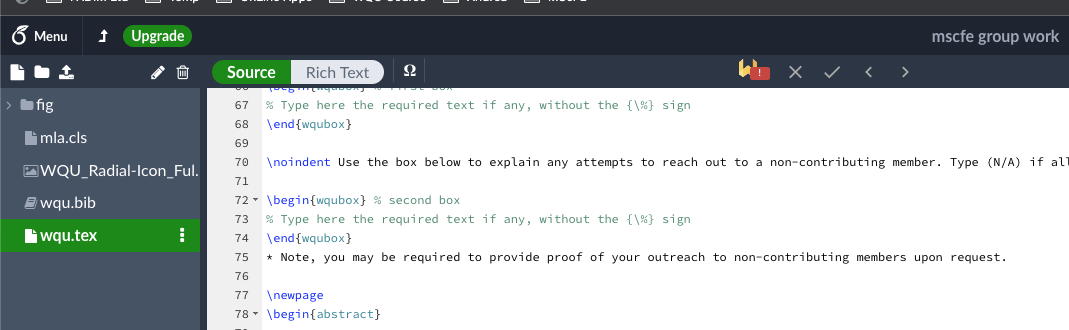
\includegraphics[width=\columnwidth]{fig/overleaf.png}
	\caption{Create a project with the name you like and copy in it the files including the fig folder.\\ Data Source: Overleaf \href{https://www.overleaf.com?r=049a7499&rm=d&rs=b}{https://www.overleaf.com}}
	\label{fig:overleaf}
\end{figure}


%TC:endignore


\section*{Section title}
The words in this section are counted. You can also add \textit{subsections}.
\subsection{ This is a subsection}
\subsubsection{This is a sub subsection}
If you want also \textit{subsubsection} are available as well as list
\begin{itemize}
    \item one
    \item two
    % sublists
    \begin{itemize}
        \item three
        \item four
    \end{itemize}
\end{itemize}



\section*{Section title two}
If you remove the asterisk after the command section they will be automatically numbered. Another citation without page number \parencite{mishkin_eakins_2018}. Please note that endnotes, references and citations are actually hyperlinks. Click on on of them, and you will go to the correct position.
If the citation is part of the context, you can use \cite[p.~32]{hull_options_2015} noted that \ldots (the command ldots inserts the ellipses, that is three dots). Now I can reuse the initial reference without any issues. \cite{mishkin_eakins_2018} observed that \ldots but if I use the same reference again it will omit the author name(s) \cite[p.~121]{mishkin_eakins_2018} observed that \ldots and you might need to manually adjust. If you have better advice, please let us know. 

A numbered list:
\begin{enumerate}
    \item one
    \item two
    \begin{enumerate}
        \item three
        \item four
    \end{enumerate}
\end{enumerate}

%TC:ignore
\section*{Conclusion}
Also the conclusion is not counted in word count. 
%TC:endignore

\end{paper}

\begin{notes}
\printendnotes
\end{notes}

\begin{workscited}
\printbibliography[heading=none]
\end{workscited}

\end{document}